\documentclass[tikz,border=5pt]{standalone}
\usepackage{fontspec}
\setmainfont{Times New Roman}
\usepackage{unicode-math}
\setmathfont{Cambria Math}
\usetikzlibrary{shapes.geometric,positioning,fit,backgrounds,arrows.meta,calc}

\begin{document}
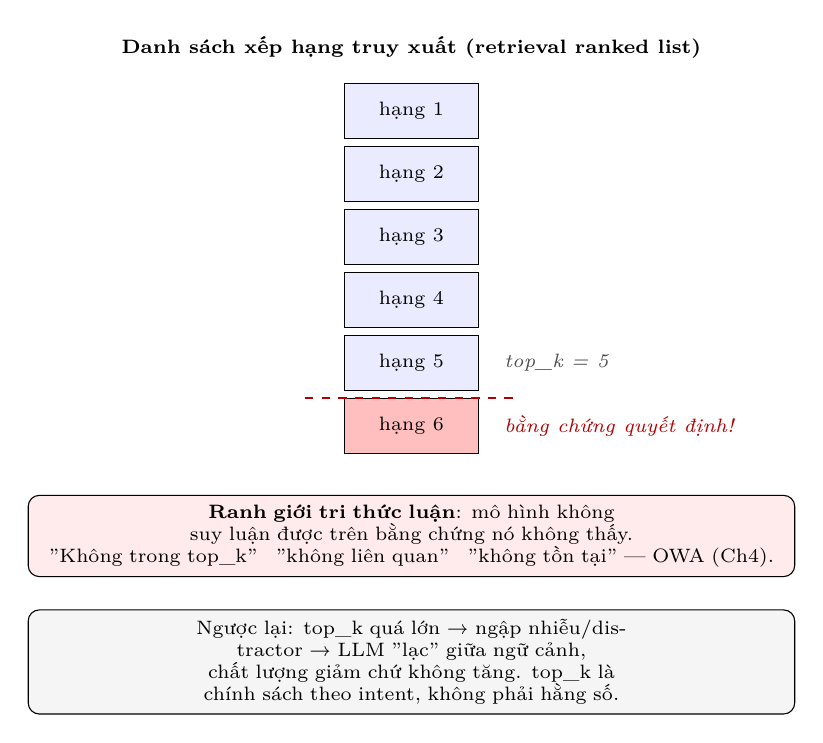
\begin{tikzpicture}[
  cell/.style={rectangle, draw, minimum width=1.7cm, minimum height=0.7cm, font=\scriptsize, align=center},
  arrow/.style={-{Stealth[length=2.2mm]}, thick},
  label/.style={font=\scriptsize\itshape, text=gray!60!black},
]

% === Ranked list with top_k boundary ===
\node[font=\scriptsize\bfseries] at (0, 2.9) {Danh sách xếp hạng truy xuất (retrieval ranked list)};

\node[cell, fill=blue!8] (r1) at (0, 2.1) {hạng 1};
\node[cell, fill=blue!8] (r2) at (0, 1.3) {hạng 2};
\node[cell, fill=blue!8] (r3) at (0, 0.5) {hạng 3};
\node[cell, fill=blue!8] (r4) at (0, -0.3) {hạng 4};
\node[cell, fill=blue!8] (r5) at (0, -1.1) {hạng 5};
\node[cell, fill=red!25] (r6) at (0, -1.9) {hạng 6};

\draw[dashed, thick, red!70!black] (-1.35, -1.55) -- (1.35, -1.55);
\node[label, right=0.2cm of r5.east] (rk) {top\_k = 5};

\node[label, right=0.2cm of r6.east, text=red!70!black] (dec) {bằng chứng quyết định!};

% === Consequence box ===
\node[draw, rounded corners, fill=red!8, align=center, font=\scriptsize, text width=9.5cm] (cons) at (0, -3.3)
  {\textbf{Ranh giới tri thức luận}: mô hình không suy luận được trên bằng chứng nó không thấy.\\
  "Không trong top\_k" ≠ "không liên quan" ≠ "không tồn tại" — OWA (Ch4).};

% === Larger k caution ===
\node[draw, rounded corners, fill=gray!8, align=center, font=\scriptsize, text width=9.5cm] (more) at (0, -4.9)
  {Ngược lại: top\_k quá lớn → ngập nhiễu/distractor → LLM "lạc" giữa ngữ cảnh,\\
  chất lượng giảm chứ không tăng. top\_k là chính sách theo intent, không phải hằng số.};

\end{tikzpicture}
\end{document}